\documentclass[11pt]{article}

\usepackage[margin=1.05in]{geometry}
\usepackage{amsmath,amssymb,amsthm}
\usepackage{graphicx}
\usepackage{enumitem}
\usepackage[round]{natbib}
\usepackage{microtype}
\usepackage{xcolor}
\usepackage{hyperref}
\hypersetup{colorlinks=true,linkcolor=blue!50!black,citecolor=blue!50!black,urlcolor=blue!50!black}

\graphicspath{{figures/}}
\setlength{\parindent}{0em}
\setlength{\parskip}{0.4em}
\setlength{\emergencystretch}{3em}

\newtheorem{proposition}{Proposition}
\newcommand{\dd}{\mathrm d}
\newcommand{\E}{\mathbb E}

\title{Intergenerational Housing Misallocation and Fertility\\[-0.1em]
\large Short model note}
\author{Tommaso De Santo}
\date{June 18, 2026}

\begin{document}
\maketitle
I set up a simplified version of the model. There are two types of agents, young and old, children require space, and a combination of a down payment friction and a tax friction generates intergenerational misallocation which impacts fertility. Results are preliminary, and proofs are omitted. The model draws inspiration from \citet{coven2024}. In this simplified version, fertility is continuous.

\section{Environment}

The economy is populated by overlapping generations of young and old households. A young household has type $i=(y_i,a_i)$: income and wealth at entry. Wealth is inherited from the previous old generation\footnote{Distributed randomly, without a tie to bequests and inheritants. It can be distributed unequally, however.}. A household decides whether to enter the economy; inside, she chooses a tenure (rent or own), a house size, completed fertility, and savings for old age. Old households, indexed by $j$, are of two kinds. Old incumbents, last period's young owners, who enter old age with financial wealth, the house they bought, and a possible accrued gain, choose how much of the house to keep and how large an estate to leave, then exit. The other type is old renters, last period's young renter entrants, who rent in old age and carry no wedge. Nonentrants stay outside the market in both periods. Each period a mass $\bar M$ of potential young households enters the pool: the maturing children of the previous cohort plus a renewal inflow. Types are distributed according to an exogenous $G_Y$.

\textbf{Preferences.} Households have preferences over consumption, housing, and children. Children raise the household's consumption and housing needs: each child claims $\chi>0$ units of consumption and $\kappa>0$ units of space, so with consumption spending $c_i$, housing $h_i$, and fertility $n_i$,
\[
u_i^Y=\log(c_i-\chi n_i)+\alpha\log(h_i-\kappa n_i)+\vartheta\log n_i .
\]
Old households value consumption, housing, and the bequest $e_j\ge0$ they leave at exit:
\[
u^O=\log c_j^O+\gamma\log h_j^O+\mathcal B(e_j),
\]
with $\mathcal B$ a warm-glow function, increasing and concave, possibly zero, common to all old households. The exiting cohort's estates are what the arriving cohort inherits. 

\textbf{Housing.} There is a fixed stock $\bar H$ of divisible floorspace, held by old incumbents and by passive absentee landlords: buyers purchase from either, renters occupy landlord space, and rents and sale proceeds are transfers.\footnote{There is no construction: the model allocates a fixed stock. This goes together with the stationary equilibrium focus. More sophisticated supply will follow in the extended model and the quantitative application.} Renting and owning are occupancy modes with different size limits, the largest sizes available to rent and to own,
\[
h\le\bar h^R \text{ (rent)},
\qquad
h\le\bar h^O \text{ (own)},
\qquad
\bar h^R<\bar h^O ,
\]
Family-sized houses are mostly available to buy, not to rent. All floorspace trades in one market: the asset price is $P$, and no-arbitrage ties the rental rate to it,
\[
q=\rho P,
\qquad
\rho=r+\delta+\tau^p .
\]
The renter pays $q$ as rent; the owner pays it as mortgage interest, property tax, depreciation, and the forgone return on her equity---different payments, equal per-unit value by arbitrage. Given $q$, a higher property tax lowers $P$ and with it the down payment on any given house.

\textbf{Financing.} A buyer finances at most a share $\phi\in(0,1)$ of the purchase, so she posts a down payment $(1-\phi)Ph$ at purchase, out of her liquid wealth. Households can save in an exogenously provided bond, but renters cannot borrow. The interest rate $r$ is exogenous.

\textbf{Taxes.} Two taxes appear: the property tax $\tau^p$, part of the user cost above, and the capital-gains tax. Selling a house triggers a tax: the seller pays the rate $\tau^g$ on the difference between the sale price and what she paid, in dollars. Dying instead passes the house with a stepped-up basis - the heir's purchase price is reset to the current value -so the gain is never taxed\footnote{This was the essence of the point suggested by Simon. I will go a bit deeper into it in the next weeks, but it is one of the two key margins (the other being financial constraints). The idea is then: agents have an incentive to hold on to the house, because this way neither they nor their heirs pay taxes.}.

Where do gains come from when the real price never moves? From inflation. Dollar prices and incomes all grow at rate $\varpi$, so relative prices and real choices are unaffected; but the tax form compares dollars from different dates, and a house bought one period ago shows a paper gain even though its real value is unchanged. The tax on that paper gain is real,
\[
\bar\ell=\tau^g\,\frac{P\,\varpi}{1+\varpi}
\]
per unit sold, and this is the model's only contact with inflation. Every cohort carries the same gain, so every incumbent's unit bears $\bar\ell$ if sold while alive.\footnote{The statutory exclusion, which exempts gains below a dollar threshold, is an institutional detail I suppress; with it, small holdings escape the tax and lock-in sorts by size.} An estate tax, by contrast, would fall on the transfer in any form and leave the sell-or-keep margin undistorted; the gains tax distorts it precisely because death forgives it. Everything is deterministic: a buyer knows the tax her future self will face \footnote{So I am resorting to a trick here to have a capital gain in a stationary model. \citet{coven2024} have a real growth term there, but they don't have my problem with fertility. More thought is required on this.}.

\section{Households}

Conditional on entry, household $i$ chooses a tenure mode $m\in\{R,O\}$, housing, fertility, consumption and savings; old age is discounted at $\beta$. For $m\in\{R,O\}$,
\[
\begin{aligned}
W_i^m=\max_{c_i,h_i,n_i,a_i'}\;&
\log(c_i-\chi n_i)+\alpha\log(h_i-\kappa n_i)+\vartheta\log n_i\\
&+\beta\big[\mathbf 1\{m=R\}\,V^R(a_{j'})+\mathbf 1\{m=O\}\,V^O(a_{j'},h_i)\big]
\end{aligned}
\]
subject to
\[
c_i+q h_i+a_i'=y_i+a_i,
\qquad
h_i\le\bar h^m,
\qquad
a_i'\ge0,
\]
\[
\mathbf 1\{m=O\}\,(1-\phi)P h_i\le a_i .
\]
Financial wealth carried into old age is $a_{j'}=(1+r)\,a_i'-\mathbf 1\{m=O\}\,q h_i$. Children have a market price: each child claims $\chi$ goods and $\kappa$ units of space, and space rents at $q$, so providing for a child costs $\chi+\kappa q$ per period. A useful benchmark is equal scaling, $\chi=\kappa q/\alpha$: the child splits her cost between space and goods in the proportion $\kappa q/\chi=\alpha$, the same proportion in which her parents split their own spending.



The old incumbent enters with financial wealth $a_j$, housing $H_j^0$, and an accrued gain; old households have no income. She faces a choice with respect to her housing: sell now and pay the tax, or keep it until death, when the tax is forgiven.\footnote{In the more realistic model we will have indivisible housing, so this will look different. With an indivisible house the choice is all-or-nothing: a strict keeper escapes the bill entirely, lock-in concentrates into a notch at the downsizing margin, and pre-saving becomes plan-contingent.} She solves
\[
\begin{aligned}
V^O(a_j,H_j^0)
&=\max_{c_j^O,\,h_j^O,\,e_j}\;u^O(c_j^O,h_j^O,e_j)
\\
&\text{subject to}\quad
c_j^O+e_j+q\,h_j^O=a_j+qH_j^0-\bar\ell\,(H_j^0-h_j^O),
\qquad
0\le h_j^O\le H_j^0 .
\end{aligned}
\]
Selling a unit nets $q-\bar\ell$; hence the stepped-up basis acts as a subsidy to locking in. An old renter has no carried housing and no tax:
\[
V^R(a_j)
=\max_{c_j^O,\,h_j^O,\,e_j}\;u^O(c_j^O,h_j^O,e_j)
\quad\text{subject to}\quad
c_j^O+e_j+q\,h_j^O=a_j,
\qquad
0<h_j^O\le\bar h^R ,
\]
and at an interior choice her marginal value of space is exactly $q$.

Using $P=q/\rho$, owner housing is bounded by
\[
H_i^O=\min\left\{\bar h^O,\;\frac{a_i\,\rho}{(1-\phi)\,q}\right\},
\qquad
H_i^R=\bar h^R .
\]
$H_i^m$ is the effective family-housing cap: a renter is capped by the stock, a buyer by the size limit or by collateral, whichever is shorter. Tenure is $W_i^Y=\max\{W_i^R,W_i^O\}$. Entry compares the inside value with an outside option $\bar W^E$ under extreme-value shocks of scale $\kappa_E$:
\[
\pi_i^E=\frac{\exp\{W_i^Y/\kappa_E\}}{\exp\{W_i^Y/\kappa_E\}+\exp\{\bar W^E/\kappa_E\}}
\]
is the probability that household $i$ enters.

\section{Equilibrium}

Aggregate demand adds young households, old incumbents, and old renters, and the single market clears:
\[
\bar M\int\pi_i^E\,h_i\,\dd G_Y(i)+\int h_j^O\,\dd F_O(j)+\int h_j^O\,\dd F_R(j)=\bar H ,
\]
where $F_O$ and $F_R$ are the measures of old incumbents and old renters.
A stationary equilibrium consists of a user cost $q$ (and $P=q/\rho$), young policies and entry probabilities, old policies, and stationary objects $(\bar M,G_Y,F_O,F_R)$ such that:
\begin{enumerate}
\item the policies solve the household problems above at $q$;
\item the floorspace market clears, as displayed;
\item the population reproduces itself: young owners become the old incumbents, young renters the old renters, and births plus the renewal inflow recreate the cohort;
\end{enumerate}

\section{Equilibrium policies}

The Lagrangian for a young agent is
\[
\begin{aligned}
\mathcal L=\;&u_i^Y+\beta\,V_{j'}+\lambda_i\big(y_i+a_i-c_i-qh_i-a_i'\big)\\
&+\mu_i\big(a_i-(1-\phi)Ph_i\big)+\theta_i\big(\bar h^m-h_i\big)+\xi_i\,a_i',
\end{aligned}
\]
with $\mu_i=0$ in the rental mode and $\xi_i\ge0$ the multiplier on the no-borrowing bound $a_i'\ge0$ for a renter. 

The first-order condition for saving sets the marginal value of resources today against the return tomorrow:
\[
\frac{1}{c_i-\chi n_i}=\beta(1+r)\,\frac{1}{c_{j'}^O}+\xi_i,
\qquad
\xi_i\,a_i'=0,
\]
which for savers ($\xi_i=0$), under logarithmic old utility (warm glow $b\log e$ included) and interior old choices, collapses to a savings rule:
\[
a_i'=\beta\left(1+\gamma+b\right)(c_i-\chi n_i)+\mathbf 1\{m=O\}\,\frac{\bar\ell\,h_i}{1+r},
\]
with $\gamma$ the old housing weight and $b$ the warm-glow weight: the household saves old age's claim on adult consumption- $k\equiv\beta(1+\gamma+b)$ -plus her discounted future tax bill, so anticipating the lock-in tax is itself a savings motive. By the same conversion, a buyer pays an effective price $q^O=q+\bar\ell/(1+r)$ per unit of space---the market price plus her own discounted lock-in tax, pre-funded through savings rather than paid as a flow---while a renter pays $q$; write $q^m$ for the mode's effective price. A unit of adult consumption commits $1+k$ units of resources, one spent now and $k$ carried.

Then, with no binding constraints, with lifetime resources $w_i=y_i+a_i$,
\[
c_i-\chi n_i=\frac{w_i}{1+\alpha+\vartheta+k},
\qquad
n_i=\frac{\vartheta\,w_i}{(1+\alpha+\vartheta+k)(\chi+\kappa q^m)},
\qquad
h_i=\frac{\alpha\,w_i}{(1+\alpha+\vartheta+k)\,q^m}+\kappa n_i,
\]


Dividing the housing derivative of $\mathcal L$ by the consumption derivative, $\lambda_i=1/(c_i-\chi n_i)$, prices every multiplier in goods. For a renter this gives
\[
\frac{\alpha\,(c_i^R-\chi n_i^R)}{h_i^R-\kappa n_i^R}=q+\zeta_i^R,
\qquad
\zeta_i^R=\frac{\theta_i}{\lambda_i}\ge0 :
\]
the left side is $u_h/u_c$, her marginal rate of substitution between space and consumption---the goods she would give up for one more unit of space, holding utility fixed---and it exceeds the rent exactly by the bite of the rental size limit, computable from her observed bundle. For a young owner the same two derivatives give
\[
\frac{\alpha\,(c_i^O-\chi n_i^O)}{h_i^O-\kappa n_i^O}=q^O+\zeta_i^O,
\qquad
\zeta_i^O=\underbrace{\frac{\mu_i}{\lambda_i}(1-\phi)P}_{\zeta_i^{O,F}\text{, down payment}}+\underbrace{\frac{\theta_i}{\lambda_i}}_{\text{size limit}} :
\]
her marginal value of space exceeds her effective price by the bite of whichever access constraints bind---the down payment ($\mu_i$) or the owner size limit ($\theta_i$). When the size limit is slack, the bundle identifies the financing bite alone ($F$ for financing): $\zeta_i^{O,F}$ is the observed ratio minus $q^O$. For an old incumbent at an interior retention choice,
\[
\frac{\gamma c_j^O}{h_j^O}=q-\bar\ell :
\]
she keeps marginal space she values below what the market would pay, because selling it would realize the taxable gain. Old renters carry no such wedge: their marginal value is $q$.

The solved policies give the level of fertility; the first-order condition behind them shows where housing enters it. Dividing that condition by the marginal utility of consumption prices the marginal child in goods: in either tenure,
\[
\underbrace{\frac{\vartheta\,(c_i^m-\chi n_i^m)}{n_i^m}}_{\text{willingness to pay for a marginal child}}
=\underbrace{\chi+\kappa\,(q^m+\zeta_i^m)}_{\text{full price of a child}} .
\]
A child's space requirement is priced at the household's own shadow value of space, so a binding access constraint acts as a tax of $\kappa\,\zeta_i^m$ per child. Children get more expensive exactly where family-sized space is hard to reach, with market prices unchanged.

\section{Efficiency}
This section is very preliminary, and serves as an illustration of what one can do with the wedges. 
The planner faces the economy's real constraints and nothing else: the stock, the size limits, goods feasibility, and the domain conditions. It does not face household budgets, since allocations are supported by lump-sum transfers, and it does not face the financing inequalities, which restrict market purchases rather than occupancy.

\begin{proposition}
Hold the stationary cross-section, entry, tenure assignments, and savings fixed; the variation below resizes two owner-occupied houses and converts no tenures. The planner's surplus from moving one unit of space from an old incumbent at an interior retention choice to a young owner whose owner size limit is slack and whose financing constraint binds ($\zeta_i^{O,F}>0$) is
\[
\underbrace{\left(q^O+\zeta_i^{O,F}\right)}_{\text{buyer's marginal value}}-\underbrace{\left(q-\bar\ell\right)}_{\text{incumbent's marginal value}}=\zeta_i^{O,F}+\frac{\bar\ell}{1+r}+\bar\ell\,>\,0 .
\]
If any constraint holds, the competitive allocation does not solve the planner's conditional problem. Conversely, if all financing gaps and levies are zero, the allocation satisfies the planner's conditional first-order conditions.
\end{proposition}

The buyer's marginal value is her effective price plus her gap: what she would pay for one more unit. The incumbent's is the net-of-tax sale price: what releasing one more unit nets her. In the difference the market price cancels, and the two tax terms that remain are transfers the planner recovers, not resource costs. If the move must be implemented through costly financing instruments rather than direct reassignment, their marginal real cost subtracts from this surplus; if the down-payment constraint is a primitive nothing relaxes, the gap is not recoverable. The long version carries this implementation cost explicitly.

Figure~\ref{fig:example} draws a solved stationary case as theory. The buyer's marginal value of space falls along her constrained path and sits above her effective price by the financing gap $\zeta^{O,F}$ at her cap, while the incumbent's sits below the market price by her tax $\bar\ell$. Pay the incumbent for one unit at her value, $q-\bar\ell$; charge the buyer at hers, $q^O+\zeta^{O,F}$: both are exactly as well off as before, and $\zeta^{O,F}+\bar\ell/(1+r)+\bar\ell$ in goods is left over.

\begin{figure}[!htb]
\centering
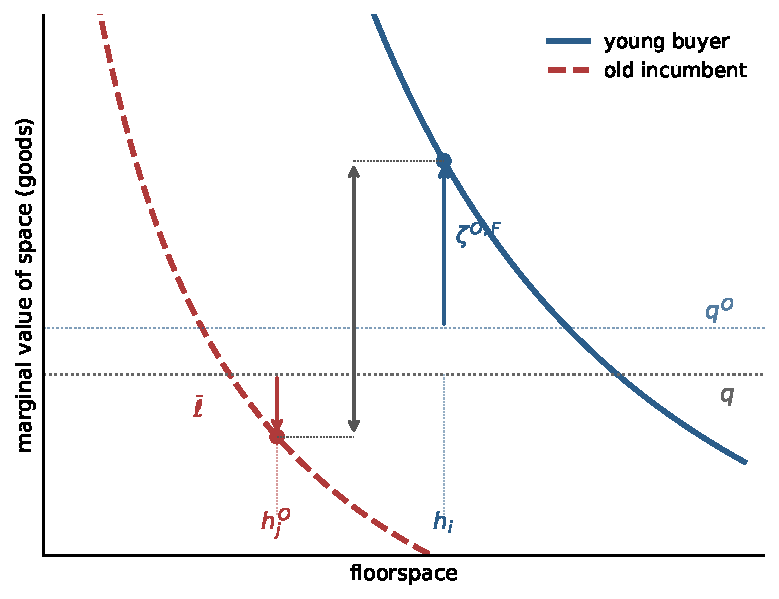
\includegraphics[width=0.58\textwidth]{example_misallocation_only.pdf}
\caption{Misallocation. The collateral-capped buyer values marginal space at $q^O+\zeta^{O,F}$, above the market price; the locked-in incumbent values it at $q-\bar\ell$, below; the distance between the two points is the recoverable surplus.}
\label{fig:example}
\end{figure}

\section{Fertility and policy}

Fix a tenure mode and a household whose cap binds, so that her housing is pinned at the effective family-housing cap of Section~2: the rental size limit for a renter, the shorter of the owner size limit and the collateral bound for a buyer. Write $H$ for the level of that cap, $w=y+a$ for lifetime resources, and $q^m$ for the mode's effective price. We relax the cap by a unit of space and study fertility. Concentrating the savings rule into the budget, fertility at the cap solves $\vartheta/n=(1+k)\chi/(w-q^mH-\chi n)+\alpha\kappa/(H-\kappa n)$; differentiating with respect to the cap level,
\[
\frac{\dd n}{\dd H}
=
\frac{\dfrac{\alpha\kappa}{(H-\kappa n)^2}-\dfrac{(1+k)\,\chi q^m}{(w-q^mH-\chi n)^2}}
{\dfrac{\vartheta}{n^2}+\dfrac{(1+k)\,\chi^2}{(w-q^mH-\chi n)^2}+\dfrac{\alpha\kappa^2}{(H-\kappa n)^2}} ,
\]
which is positive for every binding cap if and only if $\chi\le(1+k)\,\kappa q^m/\alpha$: relaxing access raises fertility whenever the child's consumption requirement does not exceed its space requirement priced at the lifetime cost of adult consumption. The derivative races two forces: extra space makes the child's space floor $\kappa$ easier to meet, pushing fertility up, while paying $q^m$ for the space tightens the budget around the child's goods floor $\chi$, pushing fertility down. The savings margin weakens the second force: the housing bill is paid partly by saving less, so only a fraction $1/(1+k)$ of it falls on current spending, and the threshold below which access raises fertility scales up by $(1+k)$. Figure~\ref{fig:fertcap} draws the relation: fertility rises along the binding cap at rate $\dd n/\dd H$ and flattens at $h^u$, where the cap stops binding.

\begin{figure}[!htb]
\centering
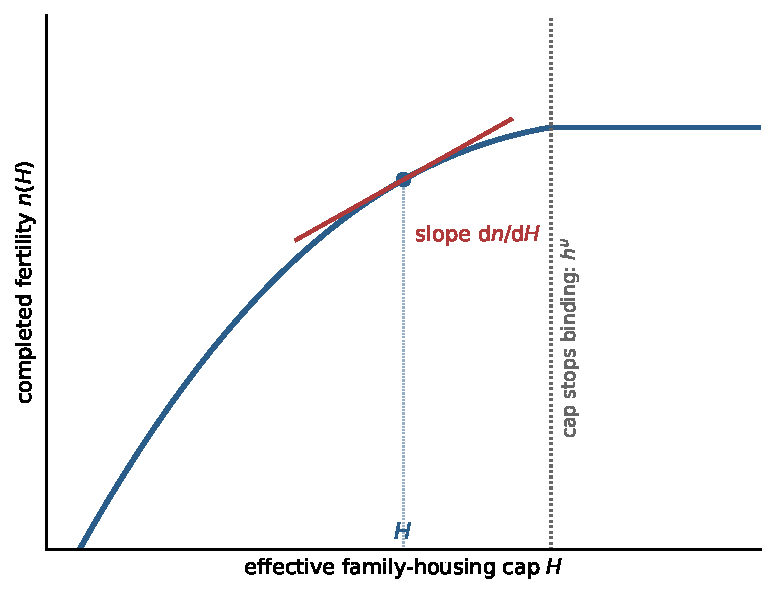
\includegraphics[width=0.58\textwidth]{example_fertility_cap.pdf}
\caption{The fertility margin. Completed fertility against the effective family-housing cap, from the same solved case as Figure~\ref{fig:example}; the slope at the equilibrium cap is $\dd n/\dd H$, and the cap stops binding at $h^u$.}
\label{fig:fertcap}
\end{figure}

One can decompose the effect of a (fertility-neutral) policy on fertility.\footnote{That is, I am not imposing here a planner solving for an explicit desired level of fertility and studying the housing channel to achieve it. Here, I am just looking at a planner who relaxes housing contraint (to ease the misallocation in Part 5) and observing that that can have a fertility impact.} The access channel runs through the cap, and the cap says where a policy can be effective: a down-payment grant raises $a_i$, financial deregulation raises $\phi$, and either loosens the collateral bound $a_i\rho/((1-\phi)q)$; making family-sized units available to rent raises $\bar h^R$. None of this is construction: the stock $\bar H$ is unchanged, and the policy changes who can occupy how much of it. At fixed prices, a small policy $z$ then moves aggregate fertility through the constrained:
\[
\left.\frac{\dd N}{\dd z}\right|_{q}
=
\bar M\sum_{m}\int_{\mathcal E_m(z)}
\left[\pi_i^E\,\Psi_i^m+n_i^m\,\frac{\pi_i^E(1-\pi_i^E)}{\kappa_E}\,\Theta_i^m\right]
\mathcal P_i^m(z)\,\dd G_Y(i),
\]
where $\mathcal E_m(z)$ is the set of households whose cap binds in mode $m$, $\mathcal P_i^m=\partial H_i^m/\partial z$ is the pass-through of the policy to the binding component of the cap, $\Psi_i^m=\dd n/\dd H$ is the fertility response, and $\Theta_i^m=\zeta_i^m/(c_i^m-\chi n_i^m)$ drives the entry term. A policy aimed at a slack constraint moves nothing: a down-payment grant does nothing for a household pinned by the rental size limit. At $\chi=(1+k)\kappa q^m/\alpha$, equal scaling at lifetime prices, $\Psi_i^m$ is proportional to $\zeta_i^m/(c_i^m-\chi n_i^m)$, so the same gap that measures misallocation predicts whose fertility responds.

Because tenure is a discrete choice, a policy that shifts $W_i^O-W_i^R$ also moves households across the rent--own boundary. The gains tax makes that crossing non-trivial. This is also explored in the forthcoming extended version.

\bibliographystyle{plainnat}
\bibliography{references}

\end{document}
